\section{Objectives}
Follow Lab 8 (PDF pages 31--34) to obtain inverter transfer curves, switching thresholds and noise margins, then test downstream regeneration using finite-duration disturbances.

\section{Specification mapping}
\begin{longtable}{p{0.31\linewidth}p{0.29\linewidth}p{0.31\linewidth}}
\toprule
Handout requirement (PDF page) & Implementation & Verification and scope \\\midrule
Step 1: VTC, slope $-1$ and NM (31--33) & 01\_dc\_transfer & Central derivative and interpolated crossings \\
Step 2: vary width ratio (32--33) & $W_p/W_n=0.75,3,12$ & All three curves \\
Step 3: noise at each ratio (33) & 02\_noise\_cascade & Positive low-state and negative high-state disturbances \\
Question: add CMOS receiver (34) & Second stage for every ratio & Both stages retained \\
\bottomrule
\end{longtable}


\section{Circuit and design derivation}
Fix $W_n=0.6\,\mu$m and $L=0.25\,\mu$m; $W_p=0.45,1.8,7.2\,\mu$m implements the three ratios. The switching threshold is defined by $V_o=V_{DD}/2$, not an individual MOS threshold. $V_{IL},V_{IH}$ are the two $dV_o/dV_i=-1$ crossings. Boundary outputs $V_{OH}=V_o(V_{IL})$ and $V_{OL}=V_o(V_{IH})$ give $NM_L=V_{IL}-V_{OL}$ and $NM_H=V_{OH}-V_{IH}$. CSV files also retain the handout's ideal-rail NM approximation to keep definitions distinct. Partial derivative tests and scattered source sizes are replaced by complete two-boundary extraction and all three ratios.

\section{Simulation setup}
This teaching rewrite uses a separately supplied model at 1.0 V and $25\,^{\circ}\mathrm C$. The specified topology, loads and comparative dimensions are retained. The handout's 2.5 V process results are not acceptance values for this model. The chosen 1 V is a simulation condition, not a verified device rating. MOS bulk terminals are explicitly connected to the corresponding supply rails.

HSPICE S-2021.09 uses RUNLVL=6, retaining waveforms, printed data and native measurements. Figures are redrawn from actual data; CSV files are in each Lab's results directory. Successful solution does not establish process reliability. Warnings from encrypted model blocks remain suppressed; the existing diagnostic did not expose actionable further details, so the warnings are not declared harmless and complete model-limit compliance is not claimed.

DC sweeps 0--1 V in 0.5 mV steps. The 18 ns transient prints every 2 ps. Low-state disturbances reach 0.2/0.4/0.48/0.6 V; high-state dips reach 0.8/0.6/0.52/0.4 V. Edges are 0.1 ns and plateaus 0.9 ns. This normalized test preserves the noise experiment without applying the original 1.2/1.3 V thresholds to a 1 V supply.

\section{Results and specification checks}
Both decks completed. Voltages and margins below are in V and use boundary output levels.
\begin{center}\small
\begin{tabular}{llllll}
\toprule
$W_p/W_n$ & $V_M$ & $V_{IL}$ & $V_{IH}$ & $NM_L$ & $NM_H$ \\
\midrule
0.75 & 0.4214 & 0.3617 & 0.4496 & 0.3237 & 0.5100 \\
3 & 0.4825 & 0.4291 & 0.5189 & 0.3855 & 0.4376 \\
12 & 0.5459 & 0.5031 & 0.5925 & 0.4600 & 0.3616 \\
\bottomrule
\end{tabular}
\end{center}

\begin{figure}[htbp]
\centering
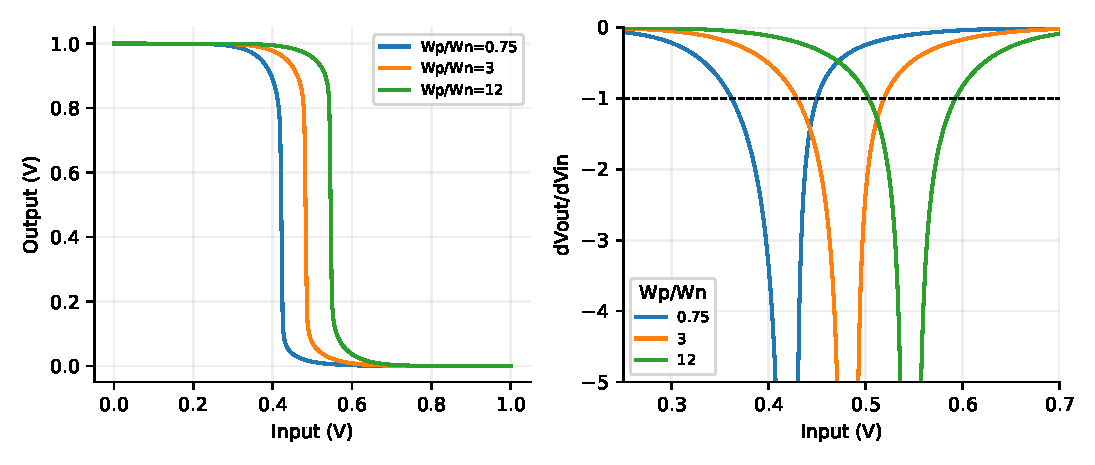
\includegraphics[width=\linewidth]{figures/inverter_transfer.pdf}
\caption{Transfer curves and unity-gain boundaries; redrawn from this run's HSPICE data.}
\end{figure}

\begin{figure}[htbp]
\centering
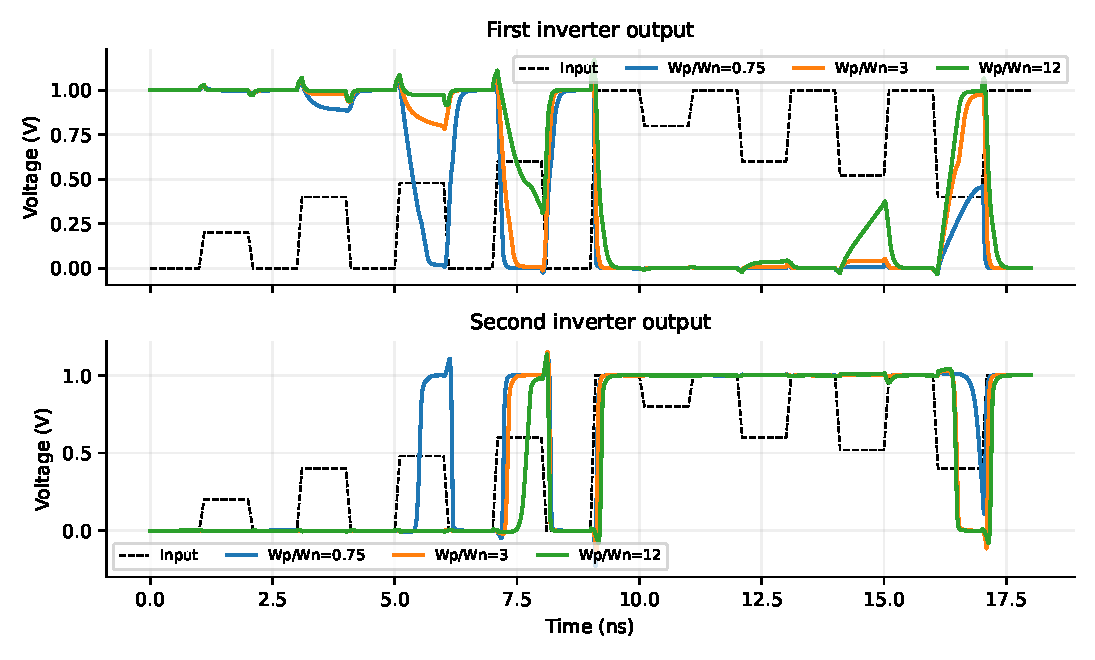
\includegraphics[width=\linewidth]{figures/noise_regeneration.pdf}
\caption{Noise responses at the first and second stages for all ratios; redrawn from this run's HSPICE data.}
\end{figure}


\section{Discussion}
Widening PMOS shifts the threshold upward, increasing $NM_L$ and decreasing $NM_H$; ratio 3 is not exactly symmetric in this model. A second stage can restore disturbances that stay outside its switching region, but may regenerate a wrong logic excursion into a full pulse. Filtering depends on duration and loading; transient survival is not identical to DC noise margin.

\section{Conclusion}
All three steps and the cascade question have complete simulation evidence. Voltage normalization and the NM definition are explicit; original-process numerical margins are not claimed.
